% Options for packages loaded elsewhere
\PassOptionsToPackage{unicode}{hyperref}
\PassOptionsToPackage{hyphens}{url}
%
\documentclass[
  ignorenonframetext,
]{beamer}
\usepackage{pgfpages}
\setbeamertemplate{caption}[numbered]
\setbeamertemplate{caption label separator}{: }
\setbeamercolor{caption name}{fg=normal text.fg}
\beamertemplatenavigationsymbolsempty
% Prevent slide breaks in the middle of a paragraph
\widowpenalties 1 10000
\raggedbottom
\setbeamertemplate{part page}{
  \centering
  \begin{beamercolorbox}[sep=16pt,center]{part title}
    \usebeamerfont{part title}\insertpart\par
  \end{beamercolorbox}
}
\setbeamertemplate{section page}{
  \centering
  \begin{beamercolorbox}[sep=12pt,center]{part title}
    \usebeamerfont{section title}\insertsection\par
  \end{beamercolorbox}
}
\setbeamertemplate{subsection page}{
  \centering
  \begin{beamercolorbox}[sep=8pt,center]{part title}
    \usebeamerfont{subsection title}\insertsubsection\par
  \end{beamercolorbox}
}
\AtBeginPart{
  \frame{\partpage}
}
\AtBeginSection{
  \ifbibliography
  \else
    \frame{\sectionpage}
  \fi
}
\AtBeginSubsection{
  \frame{\subsectionpage}
}
\usepackage{amsmath,amssymb}
\usepackage{iftex}
\ifPDFTeX
  \usepackage[T1]{fontenc}
  \usepackage[utf8]{inputenc}
  \usepackage{textcomp} % provide euro and other symbols
\else % if luatex or xetex
  \usepackage{unicode-math} % this also loads fontspec
  \defaultfontfeatures{Scale=MatchLowercase}
  \defaultfontfeatures[\rmfamily]{Ligatures=TeX,Scale=1}
\fi
\usepackage{lmodern}
\ifPDFTeX\else
  % xetex/luatex font selection
\fi
% Use upquote if available, for straight quotes in verbatim environments
\IfFileExists{upquote.sty}{\usepackage{upquote}}{}
\IfFileExists{microtype.sty}{% use microtype if available
  \usepackage[]{microtype}
  \UseMicrotypeSet[protrusion]{basicmath} % disable protrusion for tt fonts
}{}
\makeatletter
\@ifundefined{KOMAClassName}{% if non-KOMA class
  \IfFileExists{parskip.sty}{%
    \usepackage{parskip}
  }{% else
    \setlength{\parindent}{0pt}
    \setlength{\parskip}{6pt plus 2pt minus 1pt}}
}{% if KOMA class
  \KOMAoptions{parskip=half}}
\makeatother
\usepackage{xcolor}
\newif\ifbibliography
\usepackage{color}
\usepackage{fancyvrb}
\newcommand{\VerbBar}{|}
\newcommand{\VERB}{\Verb[commandchars=\\\{\}]}
\DefineVerbatimEnvironment{Highlighting}{Verbatim}{commandchars=\\\{\}}
% Add ',fontsize=\small' for more characters per line
\usepackage{framed}
\definecolor{shadecolor}{RGB}{248,248,248}
\newenvironment{Shaded}{\begin{snugshade}}{\end{snugshade}}
\newcommand{\AlertTok}[1]{\textcolor[rgb]{0.94,0.16,0.16}{#1}}
\newcommand{\AnnotationTok}[1]{\textcolor[rgb]{0.56,0.35,0.01}{\textbf{\textit{#1}}}}
\newcommand{\AttributeTok}[1]{\textcolor[rgb]{0.13,0.29,0.53}{#1}}
\newcommand{\BaseNTok}[1]{\textcolor[rgb]{0.00,0.00,0.81}{#1}}
\newcommand{\BuiltInTok}[1]{#1}
\newcommand{\CharTok}[1]{\textcolor[rgb]{0.31,0.60,0.02}{#1}}
\newcommand{\CommentTok}[1]{\textcolor[rgb]{0.56,0.35,0.01}{\textit{#1}}}
\newcommand{\CommentVarTok}[1]{\textcolor[rgb]{0.56,0.35,0.01}{\textbf{\textit{#1}}}}
\newcommand{\ConstantTok}[1]{\textcolor[rgb]{0.56,0.35,0.01}{#1}}
\newcommand{\ControlFlowTok}[1]{\textcolor[rgb]{0.13,0.29,0.53}{\textbf{#1}}}
\newcommand{\DataTypeTok}[1]{\textcolor[rgb]{0.13,0.29,0.53}{#1}}
\newcommand{\DecValTok}[1]{\textcolor[rgb]{0.00,0.00,0.81}{#1}}
\newcommand{\DocumentationTok}[1]{\textcolor[rgb]{0.56,0.35,0.01}{\textbf{\textit{#1}}}}
\newcommand{\ErrorTok}[1]{\textcolor[rgb]{0.64,0.00,0.00}{\textbf{#1}}}
\newcommand{\ExtensionTok}[1]{#1}
\newcommand{\FloatTok}[1]{\textcolor[rgb]{0.00,0.00,0.81}{#1}}
\newcommand{\FunctionTok}[1]{\textcolor[rgb]{0.13,0.29,0.53}{\textbf{#1}}}
\newcommand{\ImportTok}[1]{#1}
\newcommand{\InformationTok}[1]{\textcolor[rgb]{0.56,0.35,0.01}{\textbf{\textit{#1}}}}
\newcommand{\KeywordTok}[1]{\textcolor[rgb]{0.13,0.29,0.53}{\textbf{#1}}}
\newcommand{\NormalTok}[1]{#1}
\newcommand{\OperatorTok}[1]{\textcolor[rgb]{0.81,0.36,0.00}{\textbf{#1}}}
\newcommand{\OtherTok}[1]{\textcolor[rgb]{0.56,0.35,0.01}{#1}}
\newcommand{\PreprocessorTok}[1]{\textcolor[rgb]{0.56,0.35,0.01}{\textit{#1}}}
\newcommand{\RegionMarkerTok}[1]{#1}
\newcommand{\SpecialCharTok}[1]{\textcolor[rgb]{0.81,0.36,0.00}{\textbf{#1}}}
\newcommand{\SpecialStringTok}[1]{\textcolor[rgb]{0.31,0.60,0.02}{#1}}
\newcommand{\StringTok}[1]{\textcolor[rgb]{0.31,0.60,0.02}{#1}}
\newcommand{\VariableTok}[1]{\textcolor[rgb]{0.00,0.00,0.00}{#1}}
\newcommand{\VerbatimStringTok}[1]{\textcolor[rgb]{0.31,0.60,0.02}{#1}}
\newcommand{\WarningTok}[1]{\textcolor[rgb]{0.56,0.35,0.01}{\textbf{\textit{#1}}}}
\usepackage{graphicx}
\makeatletter
\def\maxwidth{\ifdim\Gin@nat@width>\linewidth\linewidth\else\Gin@nat@width\fi}
\def\maxheight{\ifdim\Gin@nat@height>\textheight\textheight\else\Gin@nat@height\fi}
\makeatother
% Scale images if necessary, so that they will not overflow the page
% margins by default, and it is still possible to overwrite the defaults
% using explicit options in \includegraphics[width, height, ...]{}
\setkeys{Gin}{width=\maxwidth,height=\maxheight,keepaspectratio}
% Set default figure placement to htbp
\makeatletter
\def\fps@figure{htbp}
\makeatother
\setlength{\emergencystretch}{3em} % prevent overfull lines
\providecommand{\tightlist}{%
  \setlength{\itemsep}{0pt}\setlength{\parskip}{0pt}}
\setcounter{secnumdepth}{-\maxdimen} % remove section numbering
\usepackage{amssymb}
\usepackage{hyperref}
\usepackage{multimedia}
\usepackage{graphicx}
\usepackage{xcolor}
\usepackage{tikz}
\usepackage{pgfplots}
\usepgfplotslibrary{fillbetween}
\pgfplotsset{width=10cm,compat=1.9}

\hypersetup{
	colorlinks=true,
	linkcolor=blue,
	filecolor=magenta,      
	urlcolor=cyan,
}

\urlstyle{same}

\def\begincols{\begin{columns}}
\def\begincol{\begin{column}}
\def\endcol{\end{column}}
\def\endcols{\end{columns}}

\newenvironment{stepenumerate}{\begin{enumerate}[<+->]}{\end{enumerate}}
\newenvironment{stepitemize}{\begin{itemize}[<+->]}{\end{itemize} }
\newenvironment{stepenumeratewithalert}{\begin{enumerate}[<+-| alert@+>]}{\end{enumerate}}
\newenvironment{stepitemizewithalert}{\begin{itemize}[<+-| alert@+>]}{\end{itemize} }
\usetheme{Boadilla}
\usefonttheme{serif}


%\definecolor{student}{rgb}{255, 255, 255}  % white - use for student version
\definecolor{student}{rgb}{0,0.6,0}  % green - use for full version


\ifLuaTeX
  \usepackage{selnolig}  % disable illegal ligatures
\fi
\usepackage{bookmark}
\IfFileExists{xurl.sty}{\usepackage{xurl}}{} % add URL line breaks if available
\urlstyle{same}
\hypersetup{
  pdftitle={Introduction to Handling Data},
  pdfauthor={Ralf Becker and Martyn Andrews},
  hidelinks,
  pdfcreator={LaTeX via pandoc}}

\title{Introduction to Handling Data}
\subtitle{ECON20222 - Lecture 1}
\author{Ralf Becker and Martyn Andrews}
\date{}

\begin{document}
\frame{\titlepage}

\begin{frame}{What is this course unit about?}
\phantomsection\label{what-is-this-course-unit-about}
\begin{itemize}
  \item Help you implement and interpret the main estimation and inference techniques used in Economics
  \item Focus on:
      \begin{itemize}
        \item causal inference
        \item the main pitfalls of time-series analysis
      \end{itemize}
\end{itemize}
\end{frame}

\begin{frame}{This Week's Empirical Question}
\phantomsection\label{this-weeks-empirical-question}
\begin{columns}
  
  \begin{column}{0.5\textwidth}
    \begin{figure}
        \centering
        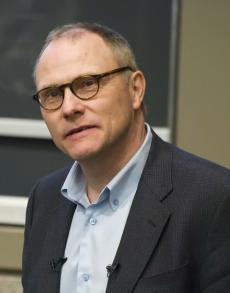
\includegraphics[width=3cm]{david-card.jpg}\\
    \end{figure}

  \end{column}
  \begin{column}{0.5\textwidth}
    \begin{figure}
        \centering
        
\includegraphics[width=3cm]{Krueger.jpeg}\\
    \end{figure}

  \end{column}
    
\end{columns}

Card, David ; Krueger, Alan B. (1994) Minimum Wages and Employment: A
Case Study of the Fast-Food Industry in New Jersey and Pennsylvania, The
American Economic Review, 84, 772-793.

Do higher minimum wages decrease employment (as predicted by
common-sense and a competitive labour market model)?
\end{frame}

\begin{frame}{The Research Question}
\phantomsection\label{the-research-question}
``This paper presents new evidence on the effect of minimum wages on
establishment-level employment outcomes. We analyze the experiences of
410 fast-food restaurants in New Jersey and Pennsylvania following the
increase in New Jersey's minimum wage from \$ 4.25 to \$ 5.05 per hour.
Comparisons of employment, wages, and prices at stores in New Jersey and
Pennsylvania before and after the rise offer a simple method for
evaluating the effects of the minimum wage.''

Card, David ; Krueger, Alan B. (1994, p.772)
\end{frame}

\begin{frame}{Why Data Matter}
\phantomsection\label{why-data-matter}
The debate is still alive:

\begin{itemize}
  \item Overall negative effect on employment, \href{https://wol.iza.org/articles/employment-effects-of-minimum-wages}{IZA}.\\
  \emph{"Research findings are not unanimous, but especially for the US, evidence suggests that minimum wages reduce the jobs available to low-skill workers."}
  \item An overview of the empirical evidence is provided in this report by \href{https://assets.publishing.service.gov.uk/government/uploads/system/uploads/attachment_data/file/844350/impacts_of_minimum_wages_review_of_the_international_evidence_Arindrajit_Dube_web.pdf}{Arindrajit Dube for the UK Government}. \\
  \emph{"Especially for the set of studies that consider broad groups of workers, the overall evidence base suggests an employment impact of close to zero."}
\end{itemize}
\end{frame}

\begin{frame}{At the end of this unit \ldots{}}
\phantomsection\label{at-the-end-of-this-unit}
You will be able to:

\begin{itemize}
  \item Understand and discuss the challenges of making causal inferences
  \item Perform inference appropriate for the model being estimated
  \item Interpret empirical results (with due caution!)
  \item Discuss strengths and weaknesses of particular empirical applications
  \item Do intermediate data work in R
  \item Confidently apply regression analysis in R
  \item Apply more advanced causal inference techniques in R
  \item Find coding help for any new challenges in R

\end{itemize}
\end{frame}

\begin{frame}{What you need to do}
\phantomsection\label{what-you-need-to-do}
To learn in this unit you need to:

\begin{figure}
    \centering
    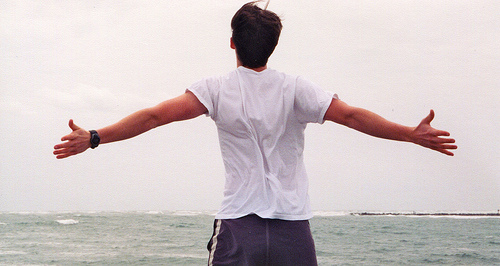
\includegraphics[width=8cm]{Embrace.jpg}\\
\end{figure}

\hfill\break

\begin{columns}
  \begin{column}{0.5\textwidth}
    \textcolor{student}{coding, cleaning data, struggling, self-learning, amazement at what you can do}
  \end{column}
  \begin{column}{0.5\textwidth}
    \textcolor{student}{answering real questions, that there is not always a clear answer}
  \end{column}
    
\end{columns}
\end{frame}

\begin{frame}{Assessment Structure and feedback}
\phantomsection\label{assessment-structure-and-feedback}
\begin{itemize}
  \item Online test (on the use of R) - 10\%
  \item End-of-Term exam (short answer questions) - 50\%
  \item Group coursework - 40\% (see extra info)

\end{itemize}
\end{frame}

\begin{frame}{Aim for today}
\phantomsection\label{aim-for-today}
\begin{columns}
  
  \begin{column}{0.5\textwidth}
    \underline{Statistics/Econometrics}
    \begin{itemize}
      \item Summary Statistics
      \item Difference between population and sample
      \item Hypothesis testing
      \item Graphical Data Representations
      \item Diff-in-Diff Analysis
      \item Simple regression analysis
    \end{itemize}
  \end{column}
  \begin{column}{0.5\textwidth}
    \underline{R Coding}
    \begin{itemize}
      \item Introduce you to R and RStudio
      \item How do I learn R
      \item Import data into R
      \item Perform some basic data manipulation
      \item Perform hypothesis tests
      \item Estimate a regression
    \end{itemize}
  \end{column}
    
\end{columns}
\end{frame}

\begin{frame}{This Week's Plan}
\phantomsection\label{this-weeks-plan}
\begin{itemize}
  \item Replicate some of the basic results presented in Card and Krueger (1994)
  \item Introduce the Difference-in-Difference methodology (Project!!) [Sometimes known as “Diff-in-Diff” or DiD.]
  \item Use this example to 
    \begin{itemize}
      \item introduce you to R
      \item review some summary statistics
      \item review simple regression and its implementation
      \item introduce some basic visualisations
    \end{itemize}
\end{itemize}
\end{frame}

\begin{frame}{Introduce R/R-Studio}
\phantomsection\label{introduce-rr-studio}
\begin{columns}
  
  \begin{column}{0.2\textwidth}
    \begin{figure}
        \centering
        
\includegraphics[width=2cm]{Rimage.jpeg}\\
    \end{figure}

  \end{column}
  \begin{column}{0.8\textwidth}
    \begin{itemize}
      \item R is a statistical software package, it is open source and free 
      \item a lot of useful functionality is added by independent researchers via packages (also for free)
    \end{itemize}
  \end{column}
    
\end{columns}

\begin{columns}
  
  \begin{column}{0.2\textwidth}
    \begin{figure}
        \centering
        
\includegraphics[width=2cm]{RStudio_image.png}\\
    \end{figure}

  \end{column}
  \begin{column}{0.8\textwidth}
    \begin{itemize}
      \item RStudio is a user interface which makes working with R easier. You need to install R before you \href{https://youtu.be/EHjakj38Nnw}{install RStudio}. 
    \end{itemize}
    
  \end{column}
    
\end{columns}

\begin{columns}
  
  \begin{column}{0.2\textwidth}
    \begin{figure}
        \centering
        
\includegraphics[width=2cm]{ECLR.jpg}\\
    \end{figure}

  \end{column}
  \begin{column}{0.8\textwidth}
    \begin{itemize}
      \item \href{https://datasquad.github.io/ECLR/}{ECLR} is a web-resource we have set up to support you in your R work. 
    \end{itemize}
    
  \end{column}
    
\end{columns}
\end{frame}

\begin{frame}{Welcome to RStudio}
\phantomsection\label{welcome-to-rstudio}
\begin{figure}
    \centering
    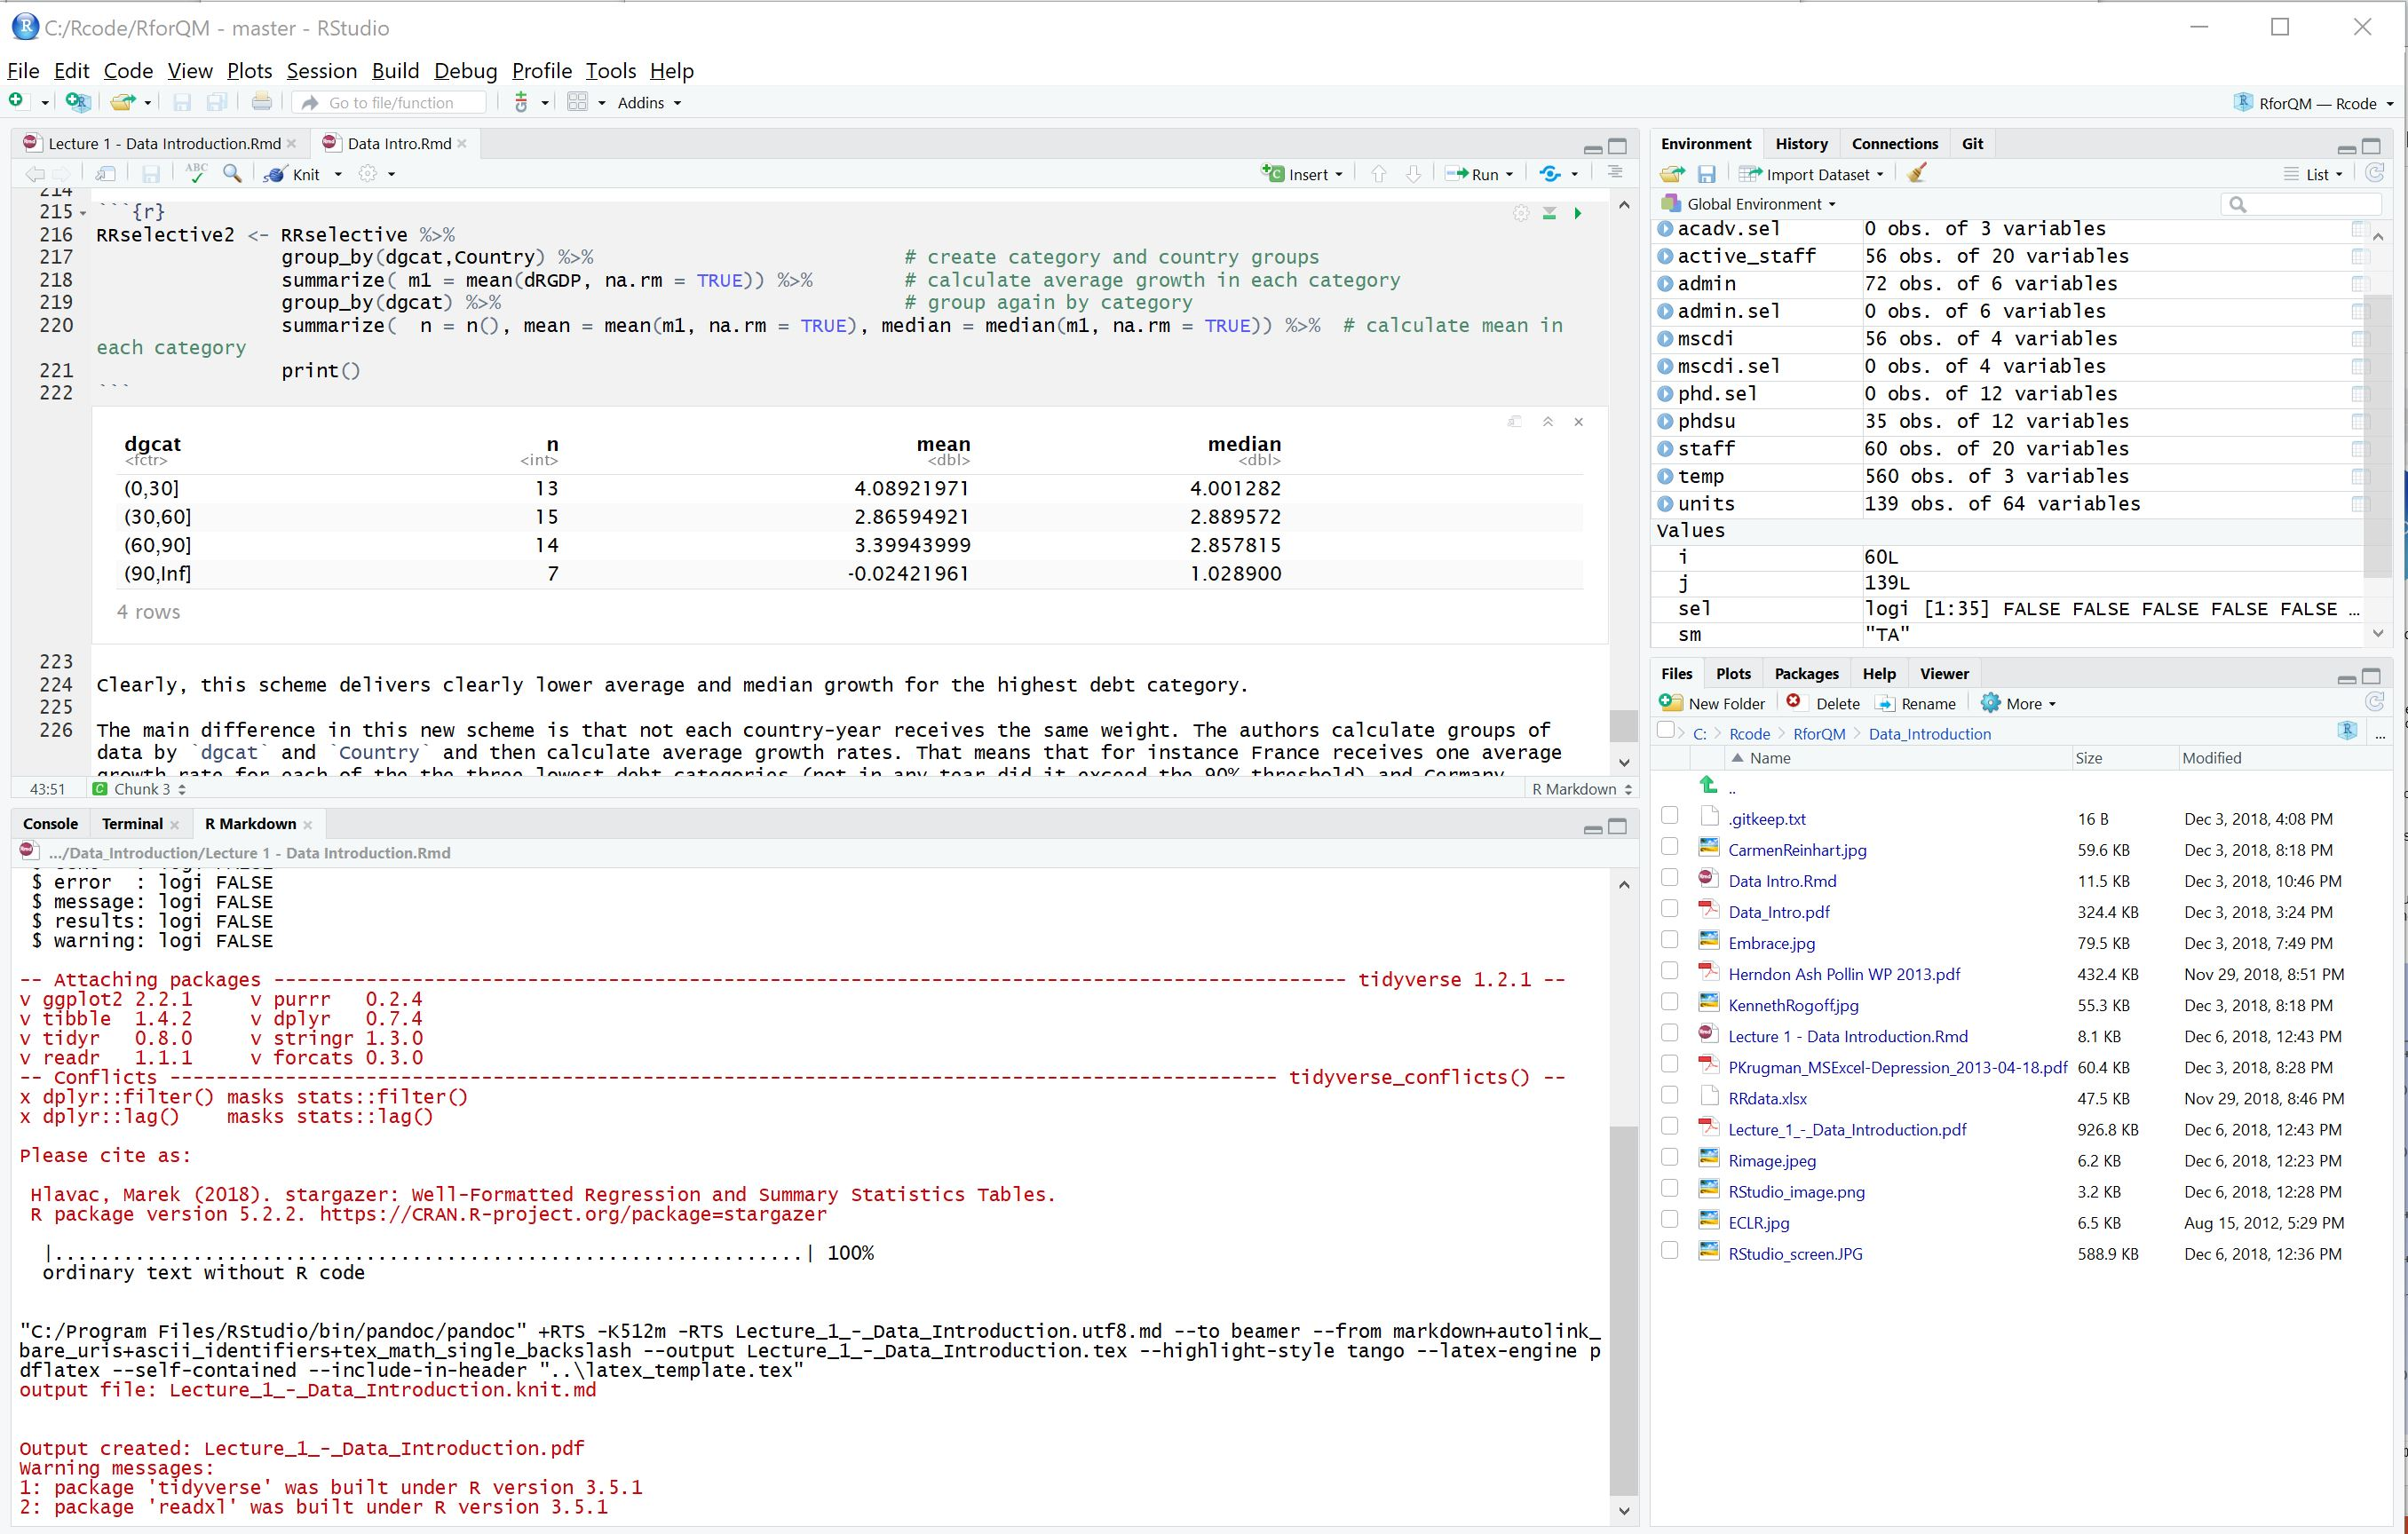
\includegraphics[width=12cm]{RStudio_screen.jpg}\\
\end{figure}
\end{frame}

\begin{frame}{Write Code Files or the Basic Workflow}
\phantomsection\label{write-code-files-or-the-basic-workflow}
\begin{itemize}
  \item keep an original data file (usually `.xlsx` or `.csv`) and do not overwrite this file
  \item any manipulation we make to the data (data cleaning, statistical analysis etc.) is command based and we collect all these commands in a script file. R will then interpret and execute these commands. It is hence like a recepie which you present to a chef. These script files have extension `.r`
  \item you can also learn to write Rmarkdown files (`.rmd`). They combine code with normal text and output. 
  \item When you write code you should ensure that you add comments to your code. Comments are bit of text which is ignored by R (everything after an `\#`) but helps you or someone else to decipher what the code does.

\end{itemize}

By following the above advice you make it easy for yourself and others
to replicate your work.
\end{frame}

\begin{frame}[fragile]{Prepare your code}
\phantomsection\label{prepare-your-code}
We start by uploading the extra packages we need in our code.

The first time you need these packages at a computer you may need to
install these. Use the following code to install packages:

\begin{Shaded}
\begin{Highlighting}[]
\FunctionTok{install.packages}\NormalTok{(}\FunctionTok{c}\NormalTok{(}\StringTok{"readxl"}\NormalTok{,}\StringTok{"tidyverse"}\NormalTok{,}\StringTok{"ggplot2"}\NormalTok{,}\StringTok{"stargazer"}\NormalTok{))}
\end{Highlighting}
\end{Shaded}

This only needs to be done once on a particular computer. However, every
time you want to use any of these packages in a code you need to make
them available to your code (load them):

\begin{Shaded}
\begin{Highlighting}[]
\FunctionTok{library}\NormalTok{(tidyverse)    }\CommentTok{\# for almost all data handling tasks}
\FunctionTok{library}\NormalTok{(readxl)       }\CommentTok{\# to import Excel data}
\FunctionTok{library}\NormalTok{(ggplot2)      }\CommentTok{\# to produce nice graphiscs}
\FunctionTok{library}\NormalTok{(stargazer)    }\CommentTok{\# to produce nice results tables}
\end{Highlighting}
\end{Shaded}
\end{frame}

\begin{frame}[fragile]{The data}
\phantomsection\label{the-data}
Then we load the data from excel

\begin{Shaded}
\begin{Highlighting}[]
\NormalTok{CKdata}\OtherTok{\textless{}{-}} \FunctionTok{read\_xlsx}\NormalTok{(}\StringTok{"../data/CK\_public.xlsx"}\NormalTok{,}\AttributeTok{na =} \StringTok{"."}\NormalTok{)}
\end{Highlighting}
\end{Shaded}

\texttt{na = "."} indicates how missing data are coded.

Check some characteristics of the data which are now stored in
\texttt{CKdata}:
\textcolor{student}{Discuss data.frame, number of obs and number of variables, their names and variable types}

\scriptsize

\begin{Shaded}
\begin{Highlighting}[]
\FunctionTok{str}\NormalTok{(CKdata)  }\CommentTok{\# prints some basic info on variables}
\end{Highlighting}
\end{Shaded}

\begin{verbatim}
## tibble [410 x 46] (S3: tbl_df/tbl/data.frame)
##  $ SHEET   : num [1:410] 46 49 506 56 61 62 445 451 455 458 ...
##  $ CHAIN   : num [1:410] 1 2 2 4 4 4 1 1 2 2 ...
##  $ CO_OWNED: num [1:410] 0 0 1 1 1 1 0 0 1 1 ...
##  $ STATE   : num [1:410] 0 0 0 0 0 0 0 0 0 0 ...
##  $ SOUTHJ  : num [1:410] 0 0 0 0 0 0 0 0 0 0 ...
##  $ CENTRALJ: num [1:410] 0 0 0 0 0 0 0 0 0 0 ...
##  $ NORTHJ  : num [1:410] 0 0 0 0 0 0 0 0 0 0 ...
##  $ PA1     : num [1:410] 1 1 1 1 1 1 0 0 0 1 ...
##  $ PA2     : num [1:410] 0 0 0 0 0 0 1 1 1 0 ...
##  $ SHORE   : num [1:410] 0 0 0 0 0 0 0 0 0 0 ...
##  $ NCALLS  : num [1:410] 0 0 0 0 0 2 0 0 0 2 ...
##  $ EMPFT   : num [1:410] 30 6.5 3 20 6 0 50 10 2 2 ...
##  $ EMPPT   : num [1:410] 15 6.5 7 20 26 31 35 17 8 10 ...
##  $ NMGRS   : num [1:410] 3 4 2 4 5 5 3 5 5 2 ...
##  $ WAGE_ST : num [1:410] NA NA NA 5 5.5 5 5 5 5.25 5 ...
##  $ INCTIME : num [1:410] 19 26 13 26 52 26 26 52 13 19 ...
##  $ FIRSTINC: num [1:410] NA NA 0.37 0.1 0.15 0.07 0.1 0.25 0.25 0.15 ...
##  $ BONUS   : num [1:410] 1 0 0 1 1 0 0 0 0 0 ...
##  $ PCTAFF  : num [1:410] NA NA 30 0 0 45 0 0 0 0 ...
##  $ MEALS   : num [1:410] 2 2 2 2 3 2 2 2 1 1 ...
##  $ OPEN    : num [1:410] 6.5 10 11 10 10 10 6 0 11 11 ...
##  $ HRSOPEN : num [1:410] 16.5 13 10 12 12 12 18 24 10 10 ...
##  $ PSODA   : num [1:410] 1.03 1.01 0.95 0.87 0.87 0.87 1.04 1.05 0.73 0.94 ...
##  $ PFRY    : num [1:410] 1.03 0.9 0.74 0.82 0.77 0.77 0.88 0.84 0.73 0.73 ...
##  $ PENTREE : num [1:410] 0.52 2.35 2.33 1.79 1.65 0.95 0.94 0.96 2.32 2.32 ...
##  $ NREGS   : num [1:410] 3 4 3 2 2 2 3 6 2 4 ...
##  $ NREGS11 : num [1:410] 3 3 3 2 2 2 3 4 2 4 ...
##  $ TYPE2   : num [1:410] 1 1 1 1 1 1 1 1 1 1 ...
##  $ STATUS2 : num [1:410] 1 1 1 1 1 1 1 1 1 1 ...
##  $ DATE2   : num [1:410] 111792 111292 111292 111492 111492 ...
##  $ NCALLS2 : num [1:410] 1 NA NA NA NA NA NA 2 NA 1 ...
##  $ EMPFT2  : num [1:410] 3.5 0 3 0 28 NA 15 26 3 2 ...
##  $ EMPPT2  : num [1:410] 35 15 7 36 3 NA 18 9 12 9 ...
##  $ NMGRS2  : num [1:410] 3 4 4 2 6 NA 5 6 2 2 ...
##  $ WAGE_ST2: num [1:410] 4.3 4.45 5 5.25 4.75 NA 4.75 5 5 5 ...
##  $ INCTIME2: num [1:410] 26 13 19 26 13 26 26 26 13 13 ...
##  $ FIRSTIN2: num [1:410] 0.08 0.05 0.25 0.15 0.15 NA 0.15 0.2 0.25 0.25 ...
##  $ SPECIAL2: num [1:410] 1 0 NA 0 0 0 0 0 0 0 ...
##  $ MEALS2  : num [1:410] 2 2 1 2 2 2 2 2 2 1 ...
##  $ OPEN2R  : num [1:410] 6.5 10 11 10 10 10 6 0 11 11 ...
##  $ HRSOPEN2: num [1:410] 16.5 13 11 12 12 12 18 24 11 10.5 ...
##  $ PSODA2  : num [1:410] 1.03 1.01 0.95 0.92 1.01 NA 1.04 1.11 0.94 0.9 ...
##  $ PFRY2   : num [1:410] NA 0.89 0.74 0.79 0.84 0.84 0.86 0.84 0.84 0.73 ...
##  $ PENTREE2: num [1:410] 0.94 2.35 2.33 0.87 0.95 1.79 0.94 0.94 2.32 2.32 ...
##  $ NREGS2  : num [1:410] 4 4 4 2 2 3 3 6 4 4 ...
##  $ NREGS112: num [1:410] 4 4 3 2 2 3 3 3 3 3 ...
\end{verbatim}

\normalsize
\end{frame}

\begin{frame}[fragile]{The data}
\phantomsection\label{the-data-1}
To see the entire dataset (like in a spreadsheet):

Either click the little spreadsheet symbol next to the data.frame in the
Environment tab, or

\begin{Shaded}
\begin{Highlighting}[]
\FunctionTok{view}\NormalTok{(CKdata)  }\CommentTok{\# prints some basic info on variables}
\end{Highlighting}
\end{Shaded}
\end{frame}

\begin{frame}[fragile]{The data - Unit of observation}
\phantomsection\label{the-data---unit-of-observation}
A unit of observation is a fast food restaurant.

Say observation 27 in our dataset is a Roy Rogers (\texttt{CHAIN = 3})
store in Pennsylvania (\texttt{STATE = 0}) with 7 full time employees
(\texttt{EMPFT}), 19 part-time employees (\texttt{EMPPT}) and 4 managers
(\texttt{NMGRS}) in Feb 1992 and 17.5 in Dec

\begin{Shaded}
\begin{Highlighting}[]
\NormalTok{CKdata[}\DecValTok{27}\NormalTok{,]  }\CommentTok{\# CKdata[which rows, which columns]}
\end{Highlighting}
\end{Shaded}

\begin{verbatim}
## # A tibble: 1 x 46
##   SHEET CHAIN CO_OWNED STATE SOUTHJ CENTRALJ NORTHJ   PA1   PA2 SHORE NCALLS
##   <dbl> <dbl>    <dbl> <dbl>  <dbl>    <dbl>  <dbl> <dbl> <dbl> <dbl>  <dbl>
## 1   515     3        1     0      0        0      0     0     1     0      0
## # i 35 more variables: EMPFT <dbl>, EMPPT <dbl>, NMGRS <dbl>, WAGE_ST <dbl>,
## #   INCTIME <dbl>, FIRSTINC <dbl>, BONUS <dbl>, PCTAFF <dbl>, MEALS <dbl>,
## #   OPEN <dbl>, HRSOPEN <dbl>, PSODA <dbl>, PFRY <dbl>, PENTREE <dbl>,
## #   NREGS <dbl>, NREGS11 <dbl>, TYPE2 <dbl>, STATUS2 <dbl>, DATE2 <dbl>,
## #   NCALLS2 <dbl>, EMPFT2 <dbl>, EMPPT2 <dbl>, NMGRS2 <dbl>, WAGE_ST2 <dbl>,
## #   INCTIME2 <dbl>, FIRSTIN2 <dbl>, SPECIAL2 <dbl>, MEALS2 <dbl>, OPEN2R <dbl>,
## #   HRSOPEN2 <dbl>, PSODA2 <dbl>, PFRY2 <dbl>, PENTREE2 <dbl>, ...
\end{verbatim}

See \texttt{CK\_codebook.txt} for details on data definitions.
\end{frame}

\begin{frame}{Addressing particular variables}
\phantomsection\label{addressing-particular-variables}
If you want to call/use the entire spreadsheet/data frame/tibble then
you call \texttt{CKdata}.

But often you want to call one variable only:

\begin{itemize}
\tightlist
\item
  \texttt{CKdata\$CHAIN}, calls \texttt{CHAIN} only
\item
  \texttt{CKdata["CHAIN"]}, calls \texttt{CHAIN} only
\item
  \texttt{CKdata[2]}, calls \texttt{CHAIN} only, as it is the 2nd
  variable
\end{itemize}

And sometimes you want to call several, but not all, variables:

\begin{itemize}
\tightlist
\item
  \texttt{CKdata[c("STATE","CHAIN")]}
\end{itemize}

\texttt{c("STATE","CHAIN")} creates a list of names. \texttt{c} really
represents a function, c for concatenation.

\textbf{Also note: R is case sensitive, \texttt{CHAIN} $\neq$ \texttt{Chain}}
\end{frame}

\begin{frame}{Variable types}
\phantomsection\label{variable-types}
These are five basic data types.

\begin{itemize}
  \item \texttt{character: "a", "swc"}
  \item \texttt{numeric: 2, 15.5}
  \item \texttt{integer: 2L (the L tells R to store this as an integer)}
  \item \texttt{logical: TRUE, FALSE}
  \item \texttt{factor: a set number of categories}
\end{itemize}

It is important that you know and understand differences between data
types. Each variable has has a particular type and some operations only
work for particular datatypes. For instance, we need \texttt{num} or
\texttt{int} for any mathematical operations.

In our data.frame we have only \texttt{num} variable types.

We will encounter \texttt{logical} variables frequently.
\textcolor{student}{they are very powerful}
\end{frame}

\begin{frame}[fragile]{\texttt{factor} variables}
\phantomsection\label{variables}
We store categorical variables as \texttt{factor} variables.

Sometimes you need to type convert to \texttt{factor} variables.

\begin{Shaded}
\begin{Highlighting}[]
\FunctionTok{str}\NormalTok{(CKdata[}\FunctionTok{c}\NormalTok{(}\StringTok{"STATE"}\NormalTok{,}\StringTok{"CHAIN"}\NormalTok{)])  }\CommentTok{\# prints some basic info on variables}
\end{Highlighting}
\end{Shaded}

\begin{verbatim}
## tibble [410 x 2] (S3: tbl_df/tbl/data.frame)
##  $ STATE: num [1:410] 0 0 0 0 0 0 0 0 0 0 ...
##  $ CHAIN: num [1:410] 1 2 2 4 4 4 1 1 2 2 ...
\end{verbatim}

\begin{itemize}
\tightlist
\item
  \texttt{STATE}, 1 if New Jersey (NJ); 0 if Pennsylvania (Pa)
\item
  \texttt{CHAIN}, 1 = Burger King; 2 = KFC; 3 = Roy Rogers; 4 = Wendy's
\end{itemize}
\end{frame}

\begin{frame}[fragile]{\texttt{factor} variables}
\phantomsection\label{variables-1}
\footnotesize

\begin{Shaded}
\begin{Highlighting}[]
\NormalTok{CKdata}\SpecialCharTok{$}\NormalTok{STATEf }\OtherTok{\textless{}{-}} \FunctionTok{as.factor}\NormalTok{(CKdata}\SpecialCharTok{$}\NormalTok{STATE)  }
\FunctionTok{levels}\NormalTok{(CKdata}\SpecialCharTok{$}\NormalTok{STATEf) }\OtherTok{\textless{}{-}} \FunctionTok{c}\NormalTok{(}\StringTok{"Pennsylvania"}\NormalTok{,}\StringTok{"New Jersey"}\NormalTok{) }

\NormalTok{CKdata}\SpecialCharTok{$}\NormalTok{CHAINf }\OtherTok{\textless{}{-}} \FunctionTok{as.factor}\NormalTok{(CKdata}\SpecialCharTok{$}\NormalTok{CHAIN)  }
\FunctionTok{levels}\NormalTok{(CKdata}\SpecialCharTok{$}\NormalTok{CHAINf) }\OtherTok{\textless{}{-}} \FunctionTok{c}\NormalTok{(}\StringTok{"Burger King"}\NormalTok{,}\StringTok{"KFC"}\NormalTok{, }\StringTok{"Roy Rogers"}\NormalTok{, }\StringTok{"Wendy\textquotesingle{}s"}\NormalTok{) }
\end{Highlighting}
\end{Shaded}

\normalsize

\begin{itemize}
  \item \texttt{CKdata\$STATE} calls variable \texttt{STATE} in dataframe \texttt{ck\_data}
  \item \texttt{<-} assigns what is on the right \texttt{as.factor(CKdata\$STATE)} to the variable on the left \texttt{CKdata\$STATEf}
  \item \texttt{as.factor(CKdata\$STATE)} calls a function \texttt{as.factor} and applies it to \texttt{CKdata\$STATE}
\end{itemize}

\footnotesize

\begin{Shaded}
\begin{Highlighting}[]
\FunctionTok{str}\NormalTok{(CKdata[}\FunctionTok{c}\NormalTok{(}\StringTok{"STATEf"}\NormalTok{,}\StringTok{"CHAINf"}\NormalTok{)])  }\CommentTok{\# prints some basic info on variables}
\end{Highlighting}
\end{Shaded}

\begin{verbatim}
## tibble [410 x 2] (S3: tbl_df/tbl/data.frame)
##  $ STATEf: Factor w/ 2 levels "Pennsylvania",..: 1 1 1 1 1 1 1 1 1 1 ...
##  $ CHAINf: Factor w/ 4 levels "Burger King",..: 1 2 2 4 4 4 1 1 2 2 ...
\end{verbatim}

\normalsize
\end{frame}

\begin{frame}[fragile]{\texttt{factor} variables}
\phantomsection\label{variables-2}
\texttt{factor} variables are variables with discrete categories. Which
ones they are you can find out with the \texttt{levels()} function:

\begin{Shaded}
\begin{Highlighting}[]
\FunctionTok{levels}\NormalTok{(CKdata}\SpecialCharTok{$}\NormalTok{CHAINf)}
\end{Highlighting}
\end{Shaded}

\begin{verbatim}
## [1] "Burger King" "KFC"         "Roy Rogers"  "Wendy's"
\end{verbatim}
\end{frame}

\begin{frame}[fragile]{Learn more about your data}
\phantomsection\label{learn-more-about-your-data}
Use the \texttt{summary} function for some initial summary stats for
\texttt{num} or \texttt{int} variables

\begin{itemize}
\tightlist
\item
  \texttt{WAGE\_ST}, starting wage (\$/hr), Wave 1, before min wage
  increase, Feb 1992
\item
  \texttt{EMPFT}, \# full-time employees before policy implementation
\end{itemize}

\footnotesize

\begin{Shaded}
\begin{Highlighting}[]
\FunctionTok{summary}\NormalTok{(CKdata[}\FunctionTok{c}\NormalTok{(}\StringTok{"WAGE\_ST"}\NormalTok{,}\StringTok{"EMPFT"}\NormalTok{)])}
\end{Highlighting}
\end{Shaded}

\begin{verbatim}
##     WAGE_ST          EMPFT       
##  Min.   :4.250   Min.   : 0.000  
##  1st Qu.:4.250   1st Qu.: 2.000  
##  Median :4.500   Median : 6.000  
##  Mean   :4.616   Mean   : 8.203  
##  3rd Qu.:4.950   3rd Qu.:12.000  
##  Max.   :5.750   Max.   :60.000  
##  NA's   :20      NA's   :6
\end{verbatim}

\normalsize
\end{frame}

\begin{frame}[fragile]{Learn more about your data}
\phantomsection\label{learn-more-about-your-data-1}
How many obs in each state and what chains

\scriptsize

\begin{Shaded}
\begin{Highlighting}[]
\NormalTok{Tab1 }\OtherTok{\textless{}{-}}\NormalTok{ CKdata }\SpecialCharTok{\%\textgreater{}\%} \FunctionTok{group\_by}\NormalTok{(STATEf) }\SpecialCharTok{\%\textgreater{}\%} 
          \FunctionTok{summarise}\NormalTok{(}\AttributeTok{n =} \FunctionTok{n}\NormalTok{()) }\SpecialCharTok{\%\textgreater{}\%} 
          \FunctionTok{print}\NormalTok{()}
\end{Highlighting}
\end{Shaded}

\begin{verbatim}
## # A tibble: 2 x 2
##   STATEf           n
##   <fct>        <int>
## 1 Pennsylvania    79
## 2 New Jersey     331
\end{verbatim}

\begin{Shaded}
\begin{Highlighting}[]
\FunctionTok{prop.table}\NormalTok{(}\FunctionTok{table}\NormalTok{(CKdata}\SpecialCharTok{$}\NormalTok{CHAINf,CKdata}\SpecialCharTok{$}\NormalTok{STATEf,}\AttributeTok{dnn =} \FunctionTok{c}\NormalTok{(}\StringTok{"Chain"}\NormalTok{, }\StringTok{"State"}\NormalTok{)),}\AttributeTok{margin =} \DecValTok{2}\NormalTok{)}
\end{Highlighting}
\end{Shaded}

\begin{verbatim}
##              State
## Chain         Pennsylvania New Jersey
##   Burger King    0.4430380  0.4108761
##   KFC            0.1518987  0.2054381
##   Roy Rogers     0.2151899  0.2477341
##   Wendy's        0.1898734  0.1359517
\end{verbatim}

\normalsize
\end{frame}

\begin{frame}[fragile]{Scatter plot of the data}
\phantomsection\label{scatter-plot-of-the-data}
\begin{Shaded}
\begin{Highlighting}[]
\NormalTok{p1 }\OtherTok{\textless{}{-}} \FunctionTok{ggplot}\NormalTok{(CKdata,}\FunctionTok{aes}\NormalTok{(WAGE\_ST,EMPFT)) }\SpecialCharTok{+}
  \FunctionTok{geom\_point}\NormalTok{(}\AttributeTok{size=}\FloatTok{0.5}\NormalTok{) }\SpecialCharTok{+}    \CommentTok{\# this produces the scatter plot}
  \FunctionTok{geom\_smooth}\NormalTok{(}\AttributeTok{method =} \StringTok{"lm"}\NormalTok{, }\AttributeTok{se =} \ConstantTok{FALSE}\NormalTok{)  }\CommentTok{\# adds the line }
\NormalTok{p1}
\end{Highlighting}
\end{Shaded}

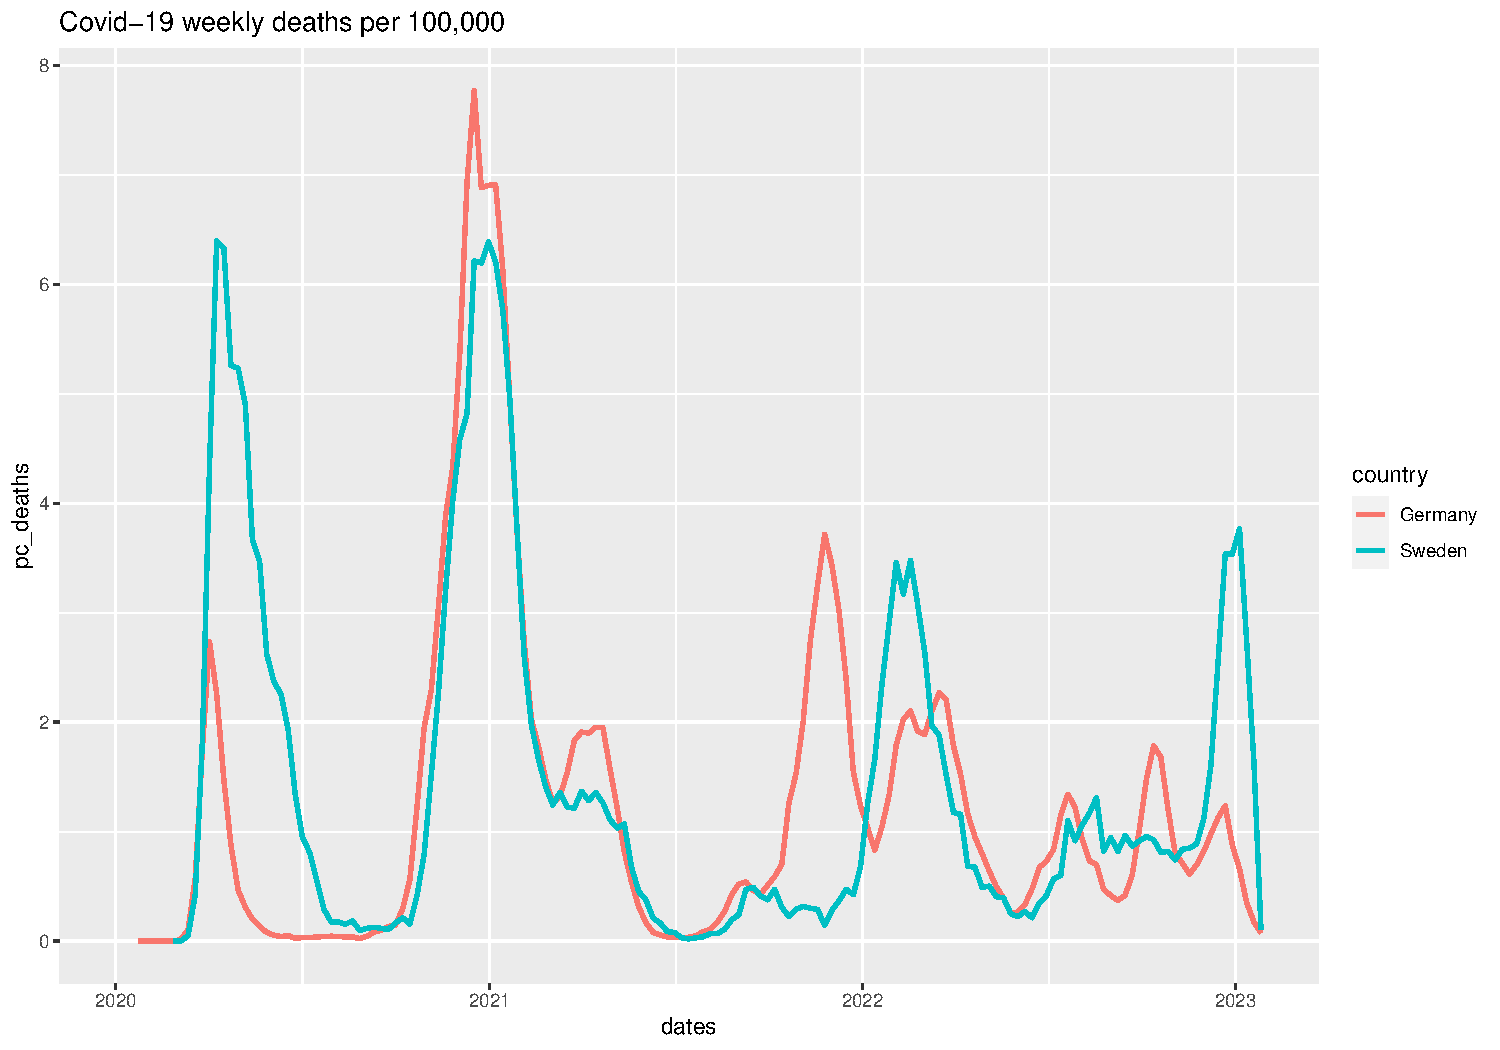
\includegraphics{Lecture-1---Data-Introduction-2025_files/figure-beamer/unnamed-chunk-14-1.pdf}

\footnotesize

\textcolor{student}{Point out that each dot represents one store data. Point out line of best fit}
\normalsize
\end{frame}

\begin{frame}{Regression Line}
\phantomsection\label{regression-line}
The line in the previous plot is the line of best fit coming from a
linear regression

\vskip -0.5cm

\[EMPFT = \alpha + \beta WAGE\_ST + u ~\text{(\textcolor{student}{Population}~~~~ Model)}\]
\vskip -0.2cm

\begin{itemize}
  \item The population model is defined by unknown parameters $\alpha$ and $\beta$ and the unknown error terms $u$. We will use sample data to obtain sample estimates of these parameters.
  \item The error terms $u$ contain the effects of any omitted variables and reflect that any modelled relationship will only be an approximation. The $u$ are \textcolor{student}{random variables}
\end{itemize}

\vskip -0.5cm

\[ EMPFT_{it} = \widehat{\alpha} + \widehat{\beta} ~ WAGE\_ST_{it} + \widehat{u}_{it} ~\text{(\textcolor{student}{Estimated Sample} ~~~~Model)}\]
\vskip -0.2cm

Here we have two subscripts as the data have a cross-section
(\texttt{\textcolor{student}{i}}) and a time-series dimension
(\texttt{\textcolor{student}{t}}).

The regression line in the previous figure is represented by
\vskip -0.5cm
\[ \widehat{EMPFT}_{it} = \widehat{\alpha} + \widehat{\beta} WAGE\_ST_{it} ~~~\text{(~~~\textcolor{student}{Regression Line}~~~~~~)}\]
\end{frame}

\begin{frame}{Simple Regression Model and OLS}
\phantomsection\label{simple-regression-model-and-ols}
Regression analysis is the core technique used in Econometrics. It is
based on certain assumptions about the \emph{Population Model} and the
error terms \(u\) (more on this in the next few weeks).

How to estimate parameters (get \(\widehat{\alpha}\) and
\(\widehat{\beta}\)) using the available sample of data? This is
typically done by Ordinary Least Squares (OLS).
\end{frame}

\begin{frame}[fragile]{Simple Regression Model and OLS}
\phantomsection\label{simple-regression-model-and-ols-1}
\footnotesize

\begin{Shaded}
\begin{Highlighting}[]
\NormalTok{mod1 }\OtherTok{\textless{}{-}} \FunctionTok{lm}\NormalTok{(EMPFT}\SpecialCharTok{\textasciitilde{}}\NormalTok{WAGE\_ST, }\AttributeTok{data=}\NormalTok{ CKdata)}
\FunctionTok{summary}\NormalTok{(mod1)}
\end{Highlighting}
\end{Shaded}

\begin{verbatim}
## 
## Call:
## lm(formula = EMPFT ~ WAGE_ST, data = CKdata)
## 
## Residuals:
##     Min      1Q  Median      3Q     Max 
## -11.091  -5.898  -2.100   3.005  51.304 
## 
## Coefficients:
##             Estimate Std. Error t value Pr(>|t|)  
## (Intercept)   -6.468      5.807  -1.114   0.2660  
## WAGE_ST        3.193      1.255   2.544   0.0114 *
## ---
## Signif. codes:  0 '***' 0.001 '**' 0.01 '*' 0.05 '.' 0.1 ' ' 1
## 
## Residual standard error: 8.5 on 383 degrees of freedom
##   (25 observations deleted due to missingness)
## Multiple R-squared:  0.01662,    Adjusted R-squared:  0.01405 
## F-statistic: 6.472 on 1 and 383 DF,  p-value: 0.01135
\end{verbatim}

\normalsize
\end{frame}

\begin{frame}{OLS - calculation and interpretation}
\phantomsection\label{ols---calculation-and-interpretation}
How were \(\widehat{\beta}\) and \(\widehat{\alpha}\) calculated?

\begin{eqnarray*}
  \widehat{\beta}&=&\dfrac{\widehat{Cov}(EMPFT_{it},WAGE\_ST_{it})}{\widehat{Var}(WAGE\_ST_{it})}\\
  \widehat{\alpha}&=&\overline{EMPFT}_{it}-\widehat{\beta}*\overline{WAGE\_ST}_{it}
\end{eqnarray*}

How to interpret \(\widehat{\beta}=3.193\)?

\textcolor{student}{An increase of one unit in \texttt{WAGE\_ST} (=USD1) is related to an increase in about 3 full time employees (\texttt{EMPFT}).}

Have we established that higher wages \textbf{cause} higher employment?

\textcolor{student}{NO}
\end{frame}

\begin{frame}{Regression Analysis - Underneath the hood}
\phantomsection\label{regression-analysis---underneath-the-hood}
Need to recognise that in a sample \(\hat{\beta}\) and \(\hat{\alpha}\)
are really \textcolor{student}{random variables}. For short
\texttt{EMPFT=E} and \texttt{WAGE\_ST=W}:

\begin{eqnarray*}
\hat{\beta} &=& \dfrac{\widehat{Cov}(E,W)}{\widehat{Var}(W)}\\
          &=&\dfrac{\widehat{Cov}(\alpha + \beta~ W + u,W)}{\widehat{Var}(W)}\\
          &=&\dfrac{\widehat{Cov}(\alpha,W) + \beta \widehat{Cov}(W,W) + \widehat{Cov}(u,W)}{\widehat{Var}(W)}\\
          &=& \beta ~\dfrac{\widehat{Var}(W)}{\widehat{Var}(W)}  + \dfrac{\widehat{Cov}(u,W)}{\widehat{Var}(W)}= \beta  + \dfrac{\widehat{Cov}(u,W)}{\widehat{Var}(W)}
\end{eqnarray*}

So \(\hat{\beta}\) is a function of the random term \(u\) and hence is
itself a random variable. Once \(\widehat{Cov}(E,W)\) and
\(\widehat{Var}(W)\) are replaced by sample estimates we get
\textcolor{student}{~ONE~} value which is draw from a
\textcolor{student}{random distribution.}
\end{frame}

\begin{frame}{OLS - estimator properties}
\phantomsection\label{ols---estimator-properties}
What can we learn from this?

\begin{itemize}
  \item If $u_{it}$ is a random variable, so is \textcolor{student}{ $\widehat{\beta}$}
  \item Any particular value we get is a \textcolor{student}{draw from a random distribution}
  \item An estimator is \textcolor{red}{unbiased} if, on average, the estimates would be equal to the unknown $\beta$\\
  \textcolor{student}{at this stage the concept of unbiasedness may still be a little hazy and that is fine}
  \item For this to happen we need to \textcolor{red}{assume} that $Cov(u,x)=0$ as then \\
        $E(\widehat{\beta})=$ \textcolor{student}{$\beta$}\\
        \textcolor{student}{Why do we need to assume this? Because while we do have values for $x_{it}$ we do not have values for the unobserved error terms $u_{it}$. Hence we cannot test this. As you will find out, this is a thinking exercise and whether it is true/false/sensible/appropriate is at the core of what we do.}
\end{itemize}
\end{frame}

\begin{frame}{OLS - the exogeneity assumption}
\phantomsection\label{ols---the-exogeneity-assumption}
For \(\widehat{\beta}\) in \(y_{it}=\alpha + \beta x_{it} + u_{it}\) to
be unbiased (i.e.~on average correct) we needed

\[Cov({u}_{it},x_{it})=0\]

This is sometimes called the \textcolor{red}{Exogeneity assumption}. The
error term has to be uncorrelated to the explanatory variable \(x_{it}\)

There are a lot of reasons why this assumption may be breached.

\begin{itemize}
  \item Simultaneity ($WAGE\_ST \rightarrow EMPFT$ and $EMPFT \rightarrow WAGE\_ST$)\\
  \footnotesize
  \textcolor{student}{Discuss the fact that we have to assume that causailty here goes in both directions. Hence we cannot attach one one-directional causal interpretation to the estimated coefficient. If you can estimate the model the other way round} \normalsize

  \item Omitted relevant variables or unobserved heterogeneity 
  \item Measurement error in $x_{it}$ 

\end{itemize}
\end{frame}

\begin{frame}{So how to make causal statements}
\phantomsection\label{so-how-to-make-causal-statements}
We can do this if we can argue/believe in the exogeneity assumption. The
methodological part of this unit introduces various standard techniques
that assume exogeneity:

\begin{itemize}
\tightlist
\item
  First Difference\\
\item
  Diff-in-Diff, to be used in Project
\item
  Instrumental Variables
\item
  Regression Discontinuity (only if time permits)
\end{itemize}

All use a generalisation of the simple regression model (above) called
the Multiple Regression Model (Week 3 following).
\end{frame}

\begin{frame}{Diff-in-Diff - The Problem}
\phantomsection\label{diff-in-diff---the-problem}
Do higher minimum wages decrease employment (as predicted by a
simplistic labour market model)?
\end{frame}

\begin{frame}{The Research Question}
\phantomsection\label{the-research-question-1}
``This paper presents new evidence on the effect of minimum wages on
establishment-level employment outcomes. We analyze the experiences of
410 fast-food restaurants in New Jersey and Pennsylvania following the
increase in New Jersey's minimum wage from \$ 4.25 to \$ 5.05 per hour.
Comparisons of employment, wages, and prices at stores in New Jersey and
Pennsylvania before and after the rise offer a simple method for
evaluating the effects of the minimum wage.''

Card, David ; Krueger, Alan B. (1994, p.772)
\end{frame}

\begin{frame}[fragile]{Wage distribution - Pre}
\phantomsection\label{wage-distribution---pre}
Look at the distribution of starting wages before the change in minimum
wage in New Jersey (\texttt{WAGE\_ST}).

At this stage it is not so important to understand the commands for
these plots.

The easiest way to plot a histogram is

\texttt{hist(CKdata\$WAGE\_ST{[}CKdata\$STATEf\ ==\ "Pennsylvania"{]})}

where, in square brackets, we select that we only want data fram
Pennsylvania.

\footnotesize

\begin{Shaded}
\begin{Highlighting}[]
\FunctionTok{hist}\NormalTok{(CKdata}\SpecialCharTok{$}\NormalTok{WAGE\_ST[CKdata}\SpecialCharTok{$}\NormalTok{STATEf }\SpecialCharTok{==} \StringTok{"Pennsylvania"}\NormalTok{])}
\FunctionTok{hist}\NormalTok{(CKdata}\SpecialCharTok{$}\NormalTok{WAGE\_ST[CKdata}\SpecialCharTok{$}\NormalTok{STATEf }\SpecialCharTok{==} \StringTok{"New Jersey"}\NormalTok{])}
\end{Highlighting}
\end{Shaded}

\normalsize
\end{frame}

\begin{frame}[fragile]{Wage distribution - Pre}
\phantomsection\label{wage-distribution---pre-1}
Or here an alternative visualisation.

\footnotesize

\begin{Shaded}
\begin{Highlighting}[]
\FunctionTok{ggplot}\NormalTok{(CKdata,}\FunctionTok{aes}\NormalTok{(WAGE\_ST, }\AttributeTok{colour =}\NormalTok{ STATEf), }\AttributeTok{colour =}\NormalTok{ STATEf) }\SpecialCharTok{+} 
    \FunctionTok{geom\_histogram}\NormalTok{(}\AttributeTok{position=}\StringTok{"identity"}\NormalTok{, }
                   \FunctionTok{aes}\NormalTok{(}\AttributeTok{y =}\NormalTok{ ..density..),}
                   \AttributeTok{bins =} \DecValTok{10}\NormalTok{,}
                   \AttributeTok{alpha =} \FloatTok{0.2}\NormalTok{) }\SpecialCharTok{+}
    \FunctionTok{ggtitle}\NormalTok{(}\FunctionTok{paste}\NormalTok{(}\StringTok{"Starting wage distribution, Feb/Mar 1992"}\NormalTok{))}
\end{Highlighting}
\end{Shaded}

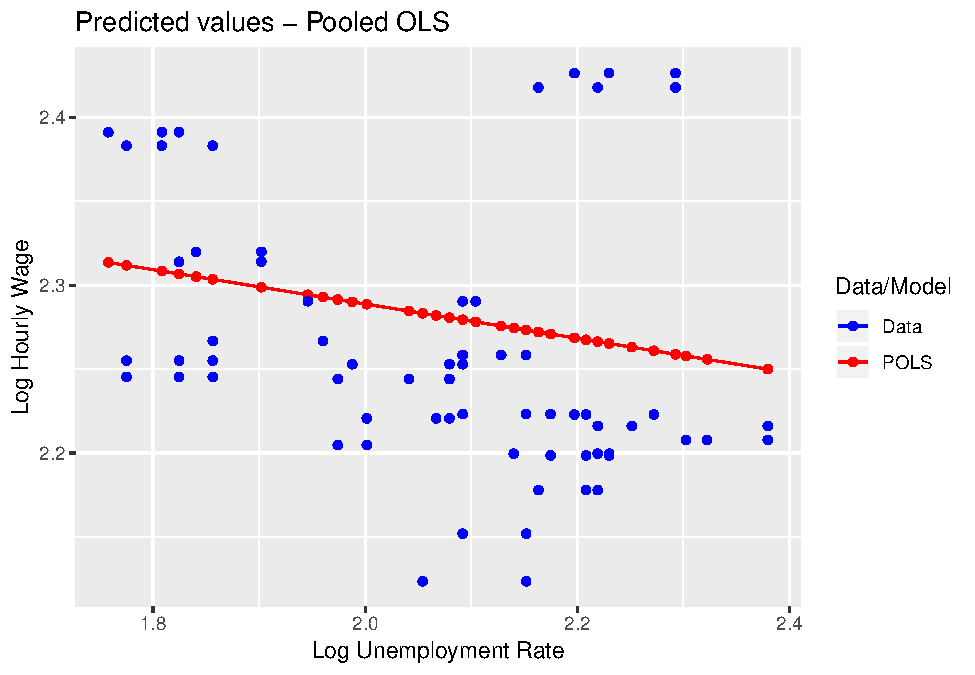
\includegraphics{Lecture-1---Data-Introduction-2025_files/figure-beamer/unnamed-chunk-17-1.pdf}
\normalsize
\end{frame}

\begin{frame}{Wage distribution - Pre}
\phantomsection\label{wage-distribution---pre-2}
Both plots show that the starting wage distribution is fairly similar in
both states, with peaks at the minimum wage of \$4.25 and \$5.00.
\end{frame}

\begin{frame}[fragile]{Policy Evaluation}
\phantomsection\label{policy-evaluation}
First we can evaluate whether the legislation has been implemented.

\footnotesize

\begin{Shaded}
\begin{Highlighting}[]
\NormalTok{Tab1 }\OtherTok{\textless{}{-}}\NormalTok{ CKdata }\SpecialCharTok{\%\textgreater{}\%} \FunctionTok{group\_by}\NormalTok{(STATEf) }\SpecialCharTok{\%\textgreater{}\%} 
          \FunctionTok{summarise}\NormalTok{(}\AttributeTok{wage\_FEB =} \FunctionTok{mean}\NormalTok{(WAGE\_ST,}\AttributeTok{na.rm =} \ConstantTok{TRUE}\NormalTok{), }
                    \AttributeTok{wage\_DEC =} \FunctionTok{mean}\NormalTok{(WAGE\_ST2,}\AttributeTok{na.rm =} \ConstantTok{TRUE}\NormalTok{)) }\SpecialCharTok{\%\textgreater{}\%} 
          \FunctionTok{print}\NormalTok{()}
\end{Highlighting}
\end{Shaded}

\begin{verbatim}
## # A tibble: 2 x 3
##   STATEf       wage_FEB wage_DEC
##   <fct>           <dbl>    <dbl>
## 1 Pennsylvania     4.63     4.62
## 2 New Jersey       4.61     5.08
\end{verbatim}

Average wage in New Jersey has increased.

\normalsize
\end{frame}

\begin{frame}[fragile]{Policy Evaluation - Wage distribution}
\phantomsection\label{policy-evaluation---wage-distribution}
\footnotesize

\begin{Shaded}
\begin{Highlighting}[]
\FunctionTok{ggplot}\NormalTok{(CKdata,}\FunctionTok{aes}\NormalTok{(WAGE\_ST2, }\AttributeTok{colour =}\NormalTok{ STATEf), }\AttributeTok{colour =}\NormalTok{ STATEf) }\SpecialCharTok{+} 
    \FunctionTok{geom\_histogram}\NormalTok{(}\AttributeTok{position=}\StringTok{"identity"}\NormalTok{, }
                   \FunctionTok{aes}\NormalTok{(}\AttributeTok{y =}\NormalTok{ ..density..),}
                   \AttributeTok{bins =} \DecValTok{10}\NormalTok{,}
                   \AttributeTok{alpha =} \FloatTok{0.2}\NormalTok{) }\SpecialCharTok{+}
    \FunctionTok{ggtitle}\NormalTok{(}\FunctionTok{paste}\NormalTok{(}\StringTok{"Starting wage distribution, Nov/Dec 1992"}\NormalTok{))}
\end{Highlighting}
\end{Shaded}

\includegraphics{Lecture-1---Data-Introduction-2025_files/figure-beamer/unnamed-chunk-19-1.pdf}
\normalsize
\end{frame}

\begin{frame}[fragile]{Policy Evaluation - Employment outcomes}
\phantomsection\label{policy-evaluation---employment-outcomes}
Let's measure employment before and after the policy change.

Calculate two new variables \texttt{FTE} and \texttt{FTE2} (full time
employment equivalent before and after policy change)

\footnotesize

\begin{Shaded}
\begin{Highlighting}[]
\NormalTok{CKdata}\SpecialCharTok{$}\NormalTok{FTE }\OtherTok{\textless{}{-}}\NormalTok{ CKdata}\SpecialCharTok{$}\NormalTok{EMPFT }\SpecialCharTok{+}\NormalTok{ CKdata}\SpecialCharTok{$}\NormalTok{NMGRS }\SpecialCharTok{+} \FloatTok{0.5}\SpecialCharTok{*}\NormalTok{CKdata}\SpecialCharTok{$}\NormalTok{EMPPT}
\NormalTok{CKdata }\OtherTok{\textless{}{-}}\NormalTok{ CKdata }\SpecialCharTok{\%\textgreater{}\%}  \FunctionTok{mutate}\NormalTok{(}\AttributeTok{FTE2 =}\NormalTok{ EMPFT2 }\SpecialCharTok{+}\NormalTok{ NMGRS2 }\SpecialCharTok{+} \FloatTok{0.5}\SpecialCharTok{*}\NormalTok{EMPPT2)}
\end{Highlighting}
\end{Shaded}

\begin{Shaded}
\begin{Highlighting}[]
\NormalTok{TabDiD }\OtherTok{\textless{}{-}}\NormalTok{ CKdata }\SpecialCharTok{\%\textgreater{}\%} \FunctionTok{group\_by}\NormalTok{(STATEf) }\SpecialCharTok{\%\textgreater{}\%} 
          \FunctionTok{summarise}\NormalTok{(}\AttributeTok{meanFTE\_FEB =} \FunctionTok{mean}\NormalTok{(FTE,}\AttributeTok{na.rm =} \ConstantTok{TRUE}\NormalTok{), }
                    \AttributeTok{meanFTE\_DEC =} \FunctionTok{mean}\NormalTok{(FTE2,}\AttributeTok{na.rm =} \ConstantTok{TRUE}\NormalTok{)) }\SpecialCharTok{\%\textgreater{}\%} 
          \FunctionTok{print}\NormalTok{()}
\end{Highlighting}
\end{Shaded}

\begin{verbatim}
## # A tibble: 2 x 3
##   STATEf       meanFTE_FEB meanFTE_DEC
##   <fct>              <dbl>       <dbl>
## 1 Pennsylvania        23.3        21.2
## 2 New Jersey          20.4        21.0
\end{verbatim}

\normalsize
\end{frame}

\begin{frame}{Policy Evaluation - Diff-in-Diff estimator}
\phantomsection\label{policy-evaluation---diff-in-diff-estimator}
\includegraphics{Lecture-1---Data-Introduction-2025_files/figure-beamer/unnamed-chunk-22-1.pdf}
\end{frame}

\begin{frame}[fragile]{Policy Evaluation - Diff-in-Diff estimator}
\phantomsection\label{policy-evaluation---diff-in-diff-estimator-1}
\begin{Shaded}
\begin{Highlighting}[]
\FunctionTok{print}\NormalTok{(TabDiD)}
\end{Highlighting}
\end{Shaded}

\begin{verbatim}
## # A tibble: 2 x 3
##   STATEf       meanFTE_FEB meanFTE_DEC
##   <fct>              <dbl>       <dbl>
## 1 Pennsylvania        23.3        21.2
## 2 New Jersey          20.4        21.0
\end{verbatim}

Numerically the DiD estimator is calculated as follows:

(21 - 20.4) - (21.2 - 23.3) = 2.7

Later: This can be calculated using a regression approach (has some
additional advantages)
\end{frame}

\begin{frame}{DiD}
\phantomsection\label{did}
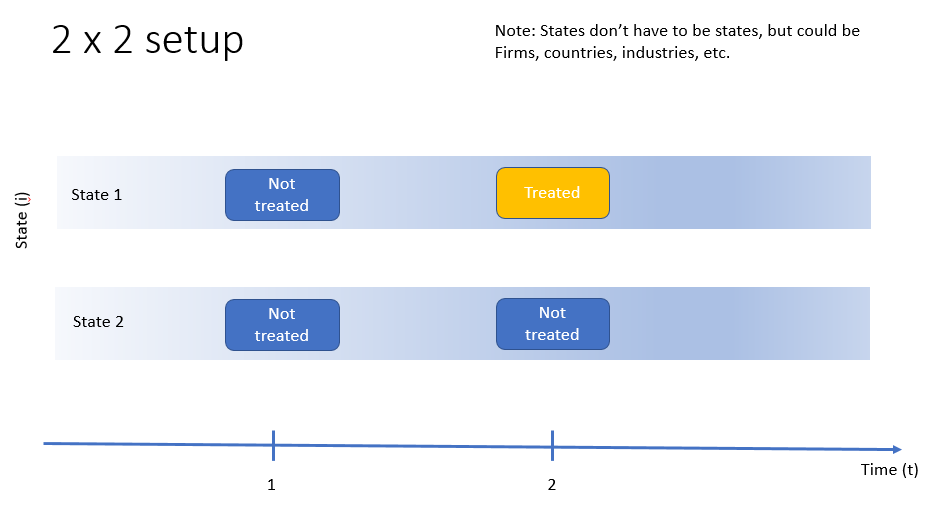
\includegraphics{2x2slide1.PNG}
\end{frame}

\begin{frame}{DiD}
\phantomsection\label{did-1}
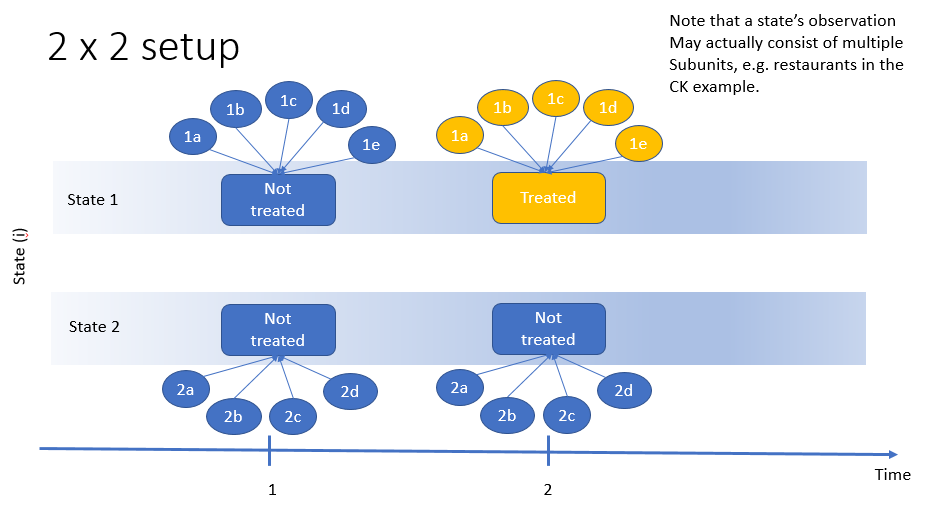
\includegraphics{2x2slide2.PNG}
\end{frame}

\begin{frame}{DiD}
\phantomsection\label{did-2}
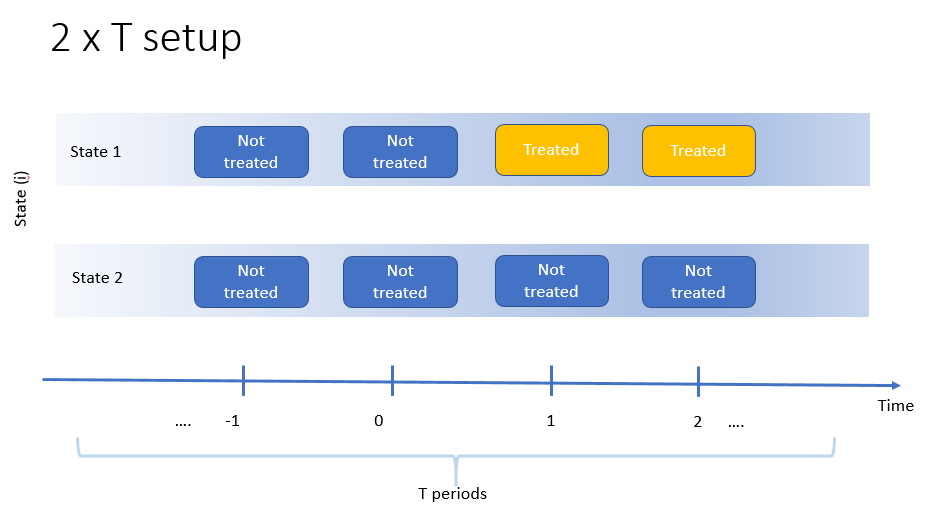
\includegraphics{2xTslide1.PNG}
\end{frame}

\begin{frame}{DiD}
\phantomsection\label{did-3}
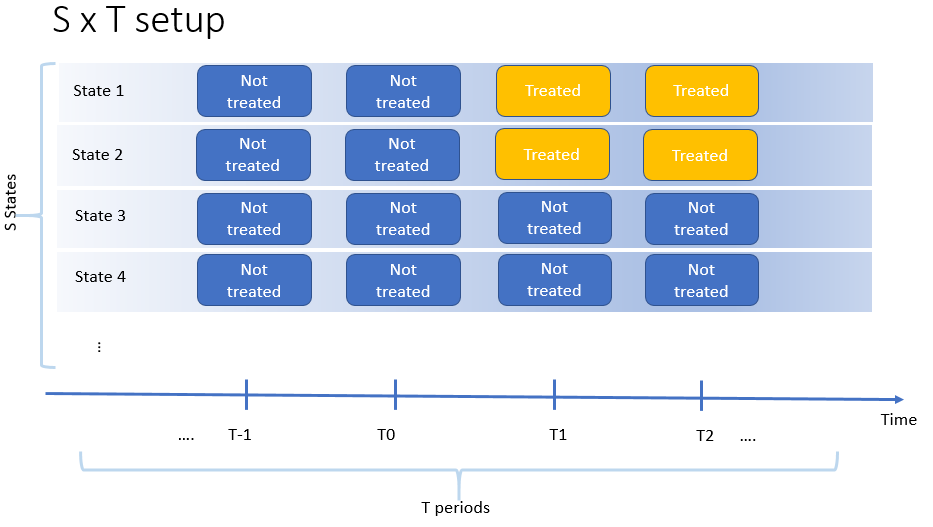
\includegraphics{2xTslide2.PNG}
\end{frame}

\begin{frame}{DiD}
\phantomsection\label{did-4}
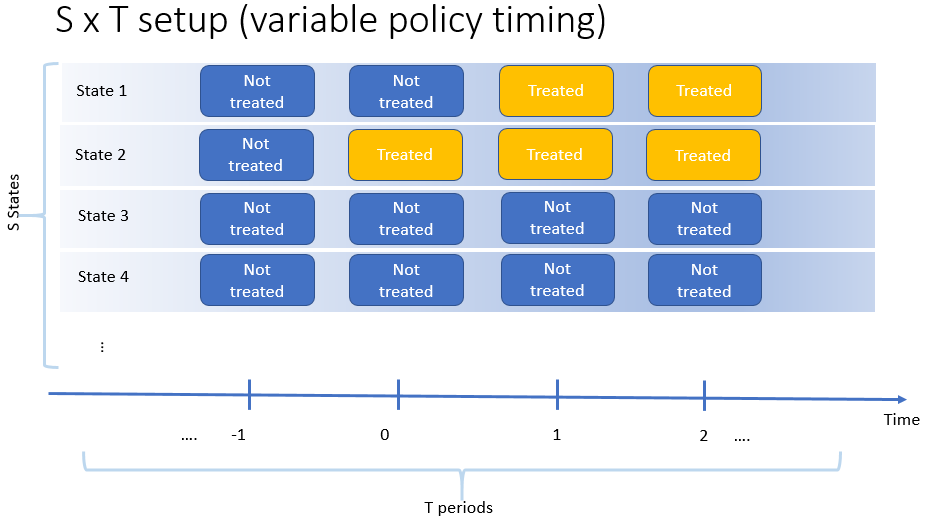
\includegraphics{2xTslide3.PNG}
\end{frame}

\begin{frame}{DiD}
\phantomsection\label{did-5}
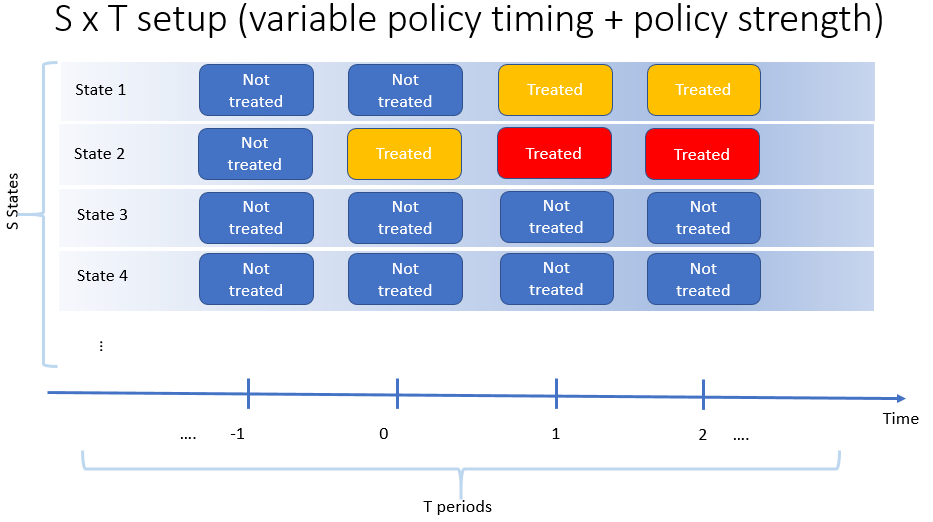
\includegraphics{2xTslide4.PNG}
\end{frame}

\begin{frame}{DiD and Regression}
\phantomsection\label{did-and-regression}
To take care of the subtleties these different schemes come with you
will have to estimate the policy effect using a regression model instead
of merely calculating averages.

Different schemes will require different setups.

This will be covered in detail in Week 7.

But here is a glimpse at one of the regression models you will come
across then

\[y_{st}=\eta + \alpha d_s + \lambda p_t + \tau d_s p_t + u_{st}\]
\end{frame}

\begin{frame}{Another Example}
\phantomsection\label{another-example}
\begin{columns}
  
  \begin{column}{0.5\textwidth}
    \small
    Siegel, M., Pahn, M., Xuan, Z., Fleegler, E. and Hemenway, D. (2019) The Impact of State Firearm Laws on Homicide and Suicide Deaths in the USA, 1991–2016: a Panel Study, J Gen Intern Med 34(10):2021–8. (available through library - see Online Reading List)\\
    \vskip 10pt
    We will develop R code to replicate this throughout the semester. This will guide you through your project.\\
    But you cannot chose this topic for your own project. And your projects will have different features
    \normalsize


  \end{column}
  \begin{column}{0.5\textwidth}
    \begin{figure}
        \centering
        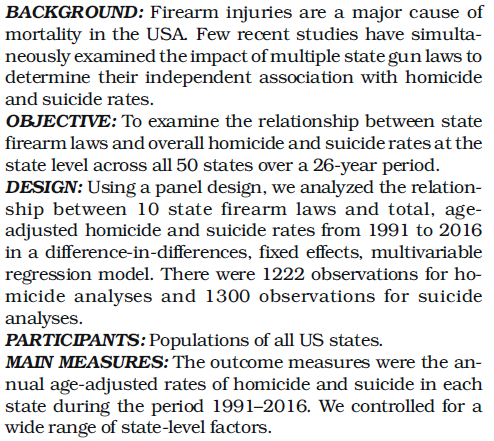
\includegraphics[width=5cm]{SiegelExtract.png}\\
    \end{figure}

  \end{column}
    
\end{columns}
\end{frame}

\begin{frame}{Outlook}
\phantomsection\label{outlook}
Over the next weeks you will learn

\begin{itemize}
  \item to perform more advanced statistical analysis in R, such as:
      \begin{itemize}
        \item Hypothesis testing
        \item Multivariate regression analysis
        \item specification testing
      \end{itemize}
  \item to devise methods to draw causal inference
  \item to understand the main pitfalls of time-series modelling and forecasting
\end{itemize}
\end{frame}

\end{document}
